\documentclass[a4paper,12pt]{article}

% Pacotes úteis
\usepackage[utf8]{inputenc}       % Codificação UTF-8
\usepackage[T1]{fontenc}          % Suporte para acentuação
\usepackage{lmodern}              % Fonte moderna
\usepackage{graphicx}             % Para inclusão de imagens
\usepackage{amsmath}              % Pacote de matemática
\usepackage{amssymb}              % Símbolos matemáticos
\usepackage{geometry}             % Controle das margens
\usepackage{setspace}             % Controle de espaçamento
\usepackage{indentfirst}          % Indentar primeiro parágrafo de cada seção
\usepackage{hyperref}             % Links clicáveis
\usepackage{float}                % Controle de posição de elementos flutuantes (figuras, tabelas)
\usepackage{titlesec}             % Personalização de títulos
         % Para imagens (caso use)
\usepackage{xcolor}           % Para cores nos textos (opcional)
\usepackage{listings}         % Para código C++ (se for incluir trechos)



\documentclass{article}
\usepackage{minted}

% Configurações opcionais para personalizar
\setminted{
    breaklines=true,      % Quebra automaticamente linhas longas
    breakanywhere=true,   % Permite quebrar palavras (opcional)
    frame=lines,          % Adiciona linhas ao redor do código
    fontsize=\small,      % Tamanho da fonte
    breaklines=true,
    breaksymbol=,         % Adiciona um símbolo (opcional)
    breakindent=10pt       % Indenta as linhas quebradas
}



% Configurações de página
% \geometry{left=3cm, right=2cm, top=2cm, bottom=2cm}
% \onehalfspacing                      % Espaçamento de 1,5 entre linhas

% % Cabeçalho com título e autores
% \title{Avaliação de LLM's na extração de dados médicos de notas clínicas}
% \author{
%     Ana Júlia Amaro Pereira Rocha \\ 
%     Maria Eduarda Mesquita Magalhães\\ 
%     Mariana Fernandes Rocha \\ 
%     Paula Eduarda de Lima \\
%     \\ Orientador: Walter Sande
% }
% \date{\today}                         % Data do relatório

% \begin{document}

% \documentclass[12pt,a4paper]{report}
\usepackage{graphicx}
\usepackage{titling}

\documentclass[a4paper,12pt]{article}

\usepackage[portuguese]{babel} % Ativa o português para hifenização
\usepackage[utf8]{inputenc}    % Suporte a caracteres acentuados
\usepackage[T1]{fontenc}       % Fonte com suporte a caracteres especiais

\begin{document}

\begin{titlepage}
    \begin{center}

        \vspace{1cm}
        \begin{minipage}{0.45\textwidth}
            \centering
            
\includegraphics[width=1.2\textwidth]{logo_fgv.png}    
        \end{minipage}
        \vspace{2cm}

        \rule{1\textwidth}{0.4pt} \\ % Linha horizontal personalizada
        \vspace{0.3cm}
        {\Huge \textbf{Projeto de Micro-Framework}} \\
        \vspace{0.2cm}
        \vspace{0.5cm}\\
        {\Large \textbf{A1 Computação Escalável}}\\
        \rule{1\textwidth}{0.4pt} % Linha horizontal personalizada


        \vspace{0.5cm}
        {\Large \textbf{FGV EMAp}} \\
        \vspace{2cm}
        
        

        
        
        % % Unidade e curso
        % {\Large \textbf{FGV EMAp}}\\[2cm]
        
        % Autores
        {\large 
            \textbf{Ana Júlia Amaro Pereira Rocha} \\ 
            \textbf{Maria Eduarda Mesquita Magalhães}\\
            \textbf{Mariana Fernandes Rocha} \\
            \textbf{Paula Eduarda de Lima}}\\[1.5cm]
        
        % Informações adicionais
        {\large 
            Ciência de Dados e Inteligência Artificial \\ 
            5º Período}\\[2cm]
        
         % Data
        \vfill
        {\large Rio de Janeiro, 2025}

        
    \end{center}
\end{titlepage}

\tableofcontents
\newpage


\section{Introdução}
Este relatório apresenta o desenvolvimento de um Micro-Framework voltado à construção de pipelines para processamento de dados. O principal objetivo é fornecer uma solução que promova maior eficiência e balanceamento de carga, por meio da execução concorrente e paralela das etapas de processamento. Embora a aplicação tenha sido especialmente construida para o monitoramento de uma doença infecciosa, sua estrutura foi projetada de forma genérica, com pontos de extensão (hot-spots) que permitem a personalização conforme as necessidades específicas de diferentes cenários.

\section{Modelagem}

\begin{figure}[H]
    \hspace{-1cm}
    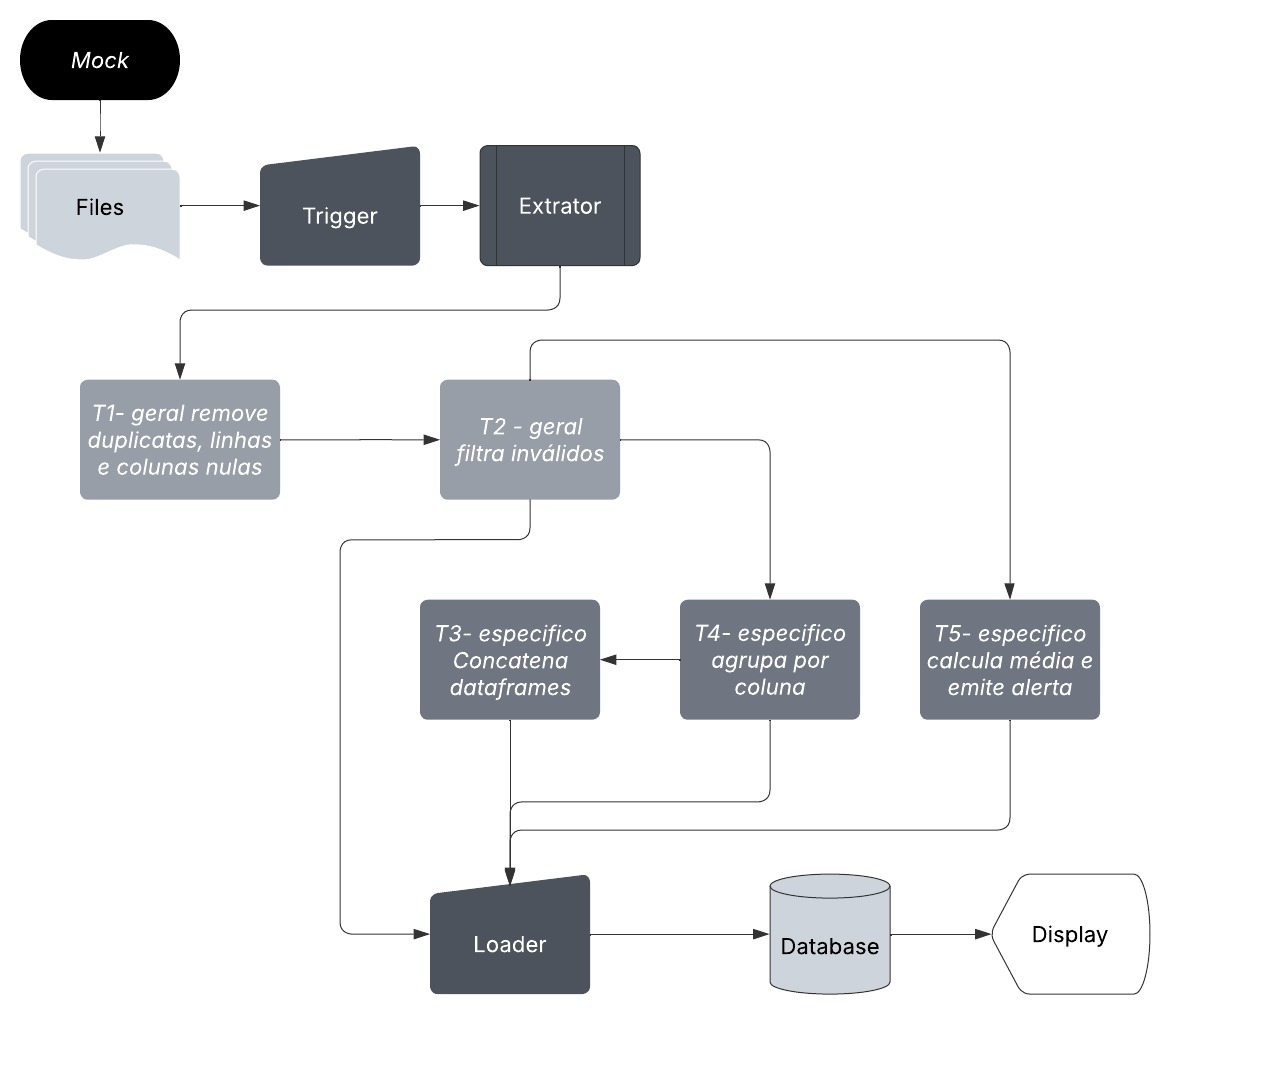
\includegraphics[width=1.15\linewidth]{Fluxograma.jpeg}
    \caption{Fluxograma do framework}
    \label{fig:minha_imagem}
\end{figure}

\section{Mock}

Nossas fontes de dados serão simulações de hospitais, da Secretaria de Saúde (SS) e da Organização Mundial da Saúde (OMS). Receberemos um conjunto de dados advindos de pelo menos uma dessas entidades toda semana. Além disso, temos dois tipos de segmentação regional: Ilhas, mais geral, e regiões, que são segmentações das ilhas, mais especifíco. A simulação apresenta 20 ilhas, cada uma identificada por um CEP de 2 dígitos, cada ilha tem 5 regiões, com CEPs de 5 dígitos, sendo os dois primeiros dígitos o CEP da ilha (ex: ilha 12 $\rightarrow$ regiões 12001 a 12005).

O objeto Mock é feito em python e implementa a criação de três tipos de tabelas diferes: SQLite, csv e txt.
\vspace{0.5cm}
\textbf{Fontes e dados gerados}

\begin{itemize}
    \item \textcolor{purple}{\textbf{OMS (\texttt{oms\_mock.txt})}}\\
    Dados agregados por ilha (CEP de 2 dígitos).\\
    Inclui número de óbitos, população, recuperados, vacinados e data.\\
    Gerado em formato \texttt{.txt} com tabulações.
    
    \vspace{0.5em}
    
    \item \textcolor{red}{\textbf{Hospitais (\texttt{hospital\_mock\_*.csv})}}\\
    Dados individuais por paciente, com CEPs de 5 dígitos (regiões).\\
    Contém informações como internação, idade, sexo, sintomas e data.\\
    Gera múltiplos arquivos \texttt{.csv}, simulando diferentes hospitais.
    
    \vspace{0.5em}
    
    \item \textcolor{orange}{\textbf{Secretaria de Saúde (\texttt{secretary\_data.db})}}\\
    Banco de dados SQLite com tabela \texttt{pacientes}.\\
    Dados por região (CEP de 5 dígitos): diagnóstico, vacinação, escolaridade, população e data.\\
    Registros inseridos diretamente em um banco relacional.
\end{itemize}

\section{Triggers}
O framework apresenta dois tipos de Triggers responsáveis por iniciar a execução de um pipeline:

\begin{itemize}
    \item \textbf{TimerTrigger}: A cada X milissegundos dispara uma nova execução.
    \item \textbf{RequestTrigger}: A cada chamada de função (simulando uma requisição de rede) dispara uma nova
execução.
\end{itemize}

\section{Extrator}

O  extrator, implementado em C++, usa a classe \texttt{DataFrame} que organiza os dados gerados pelo mock em uma estrutura tabular com colunas bem definidas e suporte a diferentes tipos de dados (inteiros, reais e strings). Ele permite:

\begin{itemize}
    \item \textbf{Validar os dados inseridos:} garante que cada valor esteja no formato correto (ex: inteiros em colunas inteiras).
    
    \item \textbf{Adicionar ou remover linhas e colunas:} facilita manipulações e atualizações nos dados carregados.
    
    \item \textbf{Visualizar os dados em forma de tabela:} com o método \texttt{display}, os dados são impressos com cabeçalho e valores formatados.
    
    \item \textbf{Acessar partes específicas:} como uma linha (\texttt{getRow}) ou coluna (\texttt{colIdx} e \texttt{typeCol}).
    
    \item \textbf{Verificar informações básicas:} número de colunas (\texttt{numCols}), número de linhas (\texttt{size}), se está vazio (\texttt{empty}), etc.
\end{itemize}

\vspace{1em}

\textbf{Aplicação com os dados gerados}
\\
\\
O extrator identifica o tipo de arquivo da tabela em questão por meio da extensão pós ponto (.csv,.txt ou .db) e, com isso, chama a respectiva função de extração para esse tipo de dado, tornando os diferentes tipos de tabelas padronizadas para o uso dos tratadores.\\
\\
Quando os dados da OMS (arquivo \texttt{.txt}) ou do hospital (arquivos \texttt{.csv}) são carregados, o \texttt{DataFrame} pode ser inicializado com os nomes das colunas e seus tipos, e cada linha é validada antes de ser inserida.
\\
\\
O extrator também pode ser usado para representar tabelas extraídas do banco de dados SQLite da Secretaria de Saúde (por exemplo, a tabela \texttt{pacientes}).
\\
\\
Ele garante integridade dos dados e fornece uma base comum para as análises posteriores.


\section{Tratadores}
\subsection{T1}
\subsection{T2}
\subsection{T3}
\subsection{T4}
\subsection{T5}
\subsection{T6}


\section{Loader}


\section{Dashboard}

\section{Pipeline}
O Pipeline é feito de modo a organizar o fluxo de trabalho de maneira eficiente e paralela. O objetivo principal é o passo a passo dejado do ETL e a escolha da ordem e dos diferentes tratadores desejados. Além disso,essa arquitetura pode ser adaptada para qualquer outro contexto de processamento de dados.

\subsection*{Lógica Produtor-Consumidor}
De maneira geral, o paralelismo no pipeline se dá pela lógica de Produtor-Consumidor, da seguinte forma:
\\
\\
\textbf{Produtor}: gera dados e os insere em uma fila compartilhada.
\\
\\
\textbf{Consumidor}: retira dados dessa fila para processá-los.
\\
\\
\textbf{Fila compartilhada}: estrutura de dados para comunicação entre threads.
\\
\\
\textbf{Mutex (trava)}: garante que só uma thread acesse a fila por vez.
\\
\\
\textbf{Condition Variable}: notifica consumidores quando há dados disponíveis (ou produtores quando há espaço, se necessário).



\subsection*{Extração}
O paralelismo na Extração dos arquivos gerados pelo mock no pipeline é implementado com base no modelo produtor-consumidor utilizando threads, filas protegidas por mutex, e variáveis de condição para sincronização.

\begin{itemize}
    \item Produtor coloca arquivos na fila (filaArquivos).

    \item  Múltiplos consumidores-extratores (threads) consomem essa fila paralelamente.

    \item  Cada consumidor-extrator:
    \begin{itemize}
        \item Lê o arquivo (pode ser .csv, .txt, ou .db).
        \item Constrói um DataFrame.
        \item Envia esse DataFrame para a próxima etapa (extratorTratadorFila), que será tratada por outra thread.
    \end{itemize}

\end{itemize}

Múltiplas threads \texttt{consumidorExtrator} são criadas (na função \texttt{executarPipeline}).

Cada thread opera de forma independente, competindo por arquivos na fila \texttt{filaArquivos}, gerando uma condição de corrida, corrigida por uma proteção da fila com mutex.
 
Isso permite que vários arquivos sejam processados \textbf{simultaneamente} por diferentes núcleos da CPU.

\subsection*{Tratamento}


\subsection*{Loader}


\subsection*{Dashboard}

\section{Análise de tempo de execução}
\end{document}
